%%%%%%%%%%%%%%%%%%%%%%%%%%%%%%%%%%%%%%%%%%%%%%%%%%%%%%%%%%%%%%%%%%%%%%%%

%%% LaTeX Template for AAMAS-2026 (based on sample-sigconf.tex)
%%% Prepared by the AAMAS-2026 Program Chairs based on the version from AAMAS-2026. 

%%%%%%%%%%%%%%%%%%%%%%%%%%%%%%%%%%%%%%%%%%%%%%%%%%%%%%%%%%%%%%%%%%%%%%%%

%%% Start your document with the \documentclass command.


%%% == IMPORTANT ==
%%% Use the first variant below for the final paper (including auithor information).
%%% Use the second variant below to anonymize your submission (no authoir information shown).
%%% For further information on anonymity and double-blind reviewing, 
%%% please consult the call for paper information
%%% https://cyprusconferences.org/aamas2026/submission-instructions/


%%%% For anonymized submission, use this
%\documentclass[sigconf,anonymous]{aamas} 

%%%% For camera-ready, use this
\documentclass[sigconf]{aamas} 


%%% Load required packages here (note that many are included already).
\usepackage{balance}
\usepackage{booktabs}
\usepackage{graphicx}
\usepackage{amsmath}
\usepackage{amsfonts}
\usepackage{amssymb}
\usepackage{array}
\usepackage{multirow}
\usepackage{url}
\usepackage{hyperref}
\usepackage{threeparttable}
\usepackage{balance} % for balancing columns on the final page

%%%%%%%%%%%%%%%%%%%%%%%%%%%%%%%%%%%%%%%%%%%%%%%%%%%%%%%%%%%%%%%%%%%%%%%%

%%% == IMPORTANT ==
%For the final camera-ready submission, you will be assigned a DOI. The DOI suffix is included in the subject line of an email sent by Sheridan, which starts with ``About your submission'' (for example: ``About your submission (aamas LT) … DOI: NIBB4567''). Copy this suffix and paste it into the \verb|\doi| command in the preamble. Do not confuse this with the \verb|\acmDOI| command in the copyright block, which must not be changed. DOIs will be registered and become active shortly after the material is published in the ACM Digital Library (estimated to be on or about the start of the event).

\doi{YDMY4904}

%%%%%%%%%%%%%%%%%%%%%%%%%%%%%%%%%%%%%%%%%%%%%%%%%%%%%%%%%%%%%%%%%%%%%%%%

%%% AAMAS-2026 copyright block (do not change!)

\makeatletter
\gdef\@copyrightpermission{
  \begin{minipage}{0.2\columnwidth}
   \href{https://creativecommons.org/licenses/by/4.0/}{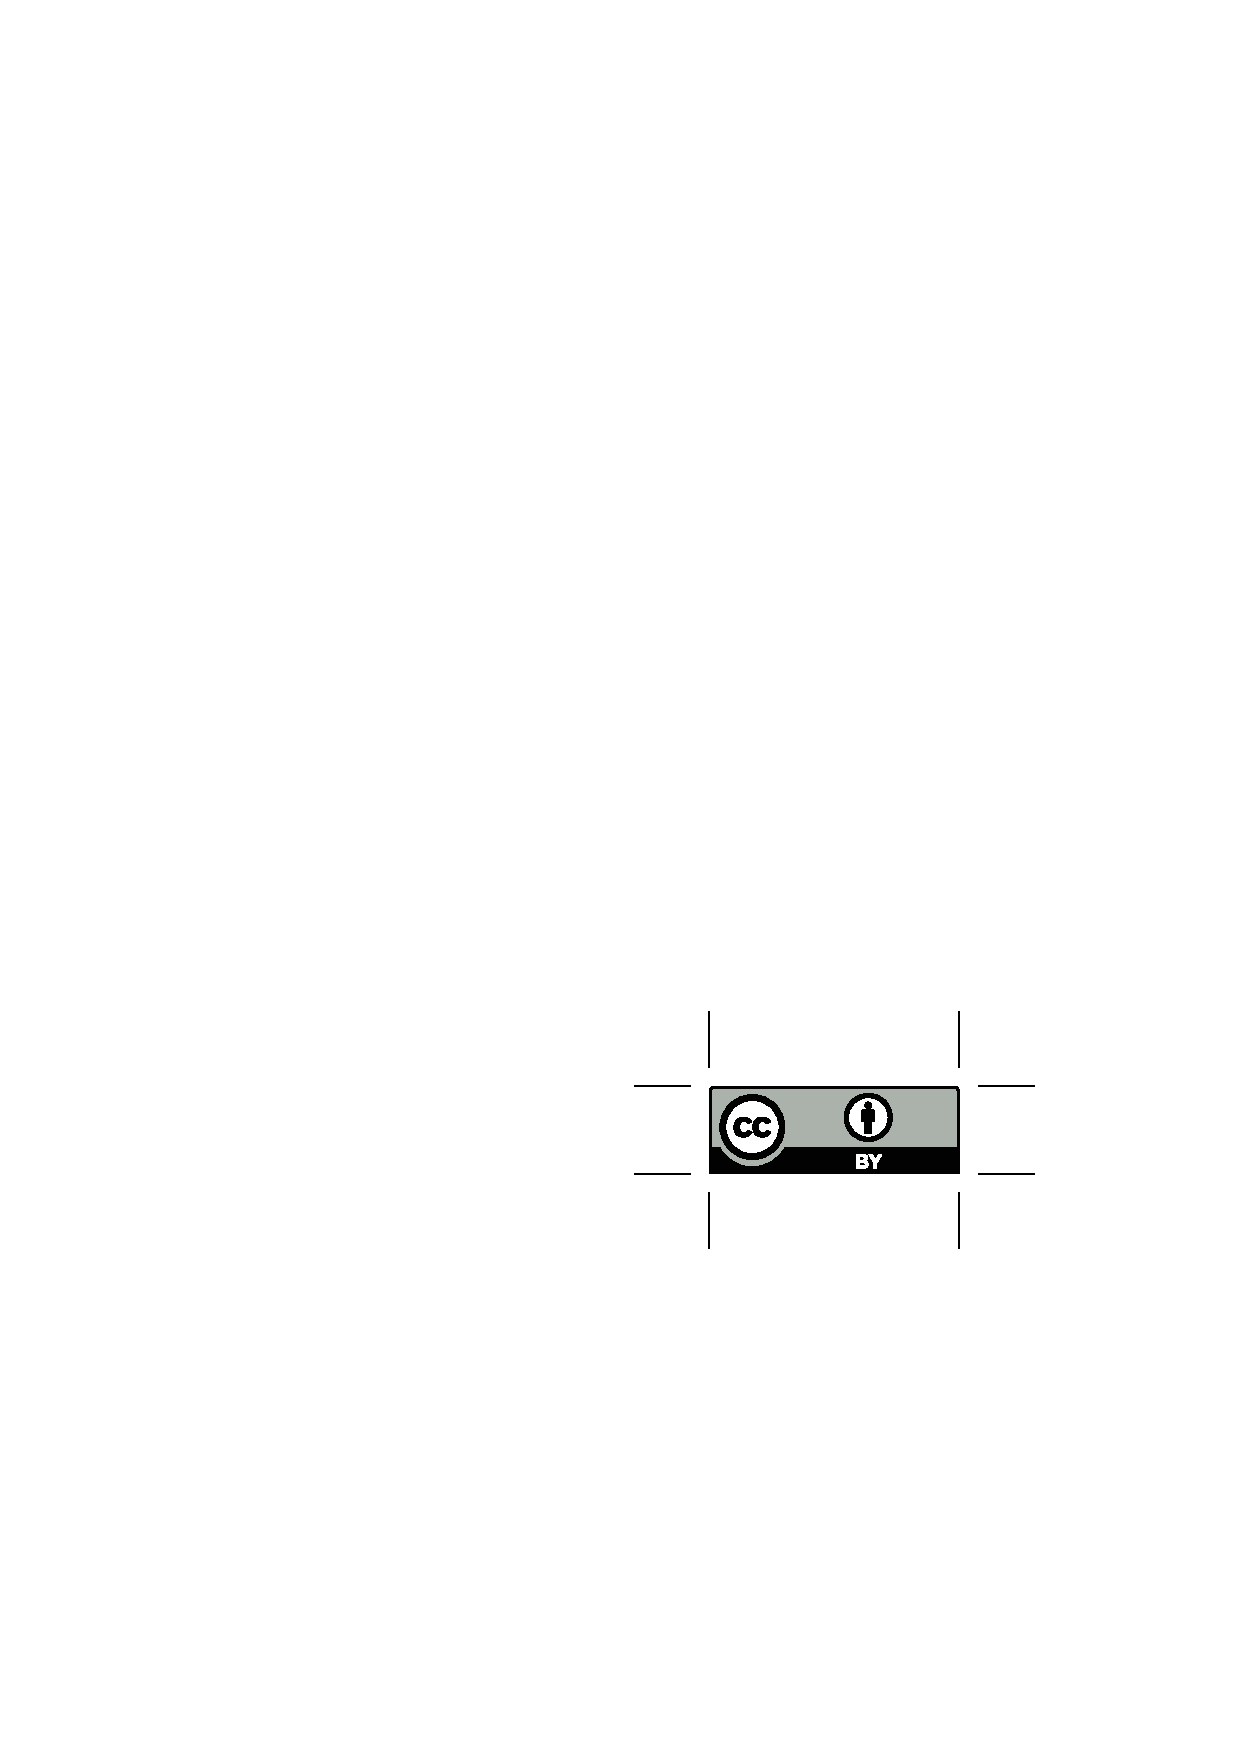
\includegraphics[width=0.90\textwidth]{by}}
  \end{minipage}\hfill
  \begin{minipage}{0.8\columnwidth}
   \href{https://creativecommons.org/licenses/by/4.0/}{This work is licensed under a Creative Commons Attribution International 4.0 License.}
  \end{minipage}
  \vspace{5pt}
}
\makeatother

\setcopyright{ifaamas}
\acmConference[AAMAS '26]{Proc.\@ of the 25th International Conference
on Autonomous Agents and Multiagent Systems (AAMAS 2026)}{May 25 -- 29, 2026}
{Paphos, Cyprus}{C.~Amato, L.~Dennis, V.~Mascardi, J.~Thangarajah (eds.)}
\copyrightyear{2026}
\acmYear{2026}
\acmDOI{}
\acmPrice{}
\acmISBN{}

%%%%%%%%%%%%%%%%%%%%%%%%%%%%%%%%%%%%%%%%%%%%%%%%%%%%%%%%%%%%%%%%%%%%%%%%

%%% == IMPORTANT ==
%%% Use this command to specify your OpenReview submission number.
%%% In anonymous mode, it will be printed on the first page.

% \acmSubmissionID{10}

%%% Use this command to specify the title of your paper.

\title{ConvPayMAS: Conversational Payment Multi-Agent System with Agent-to-Agent Protocol and Three-Mandate Verification}

% Add the subtitle below for an extended abstract
% \subtitle{Extended Abstract}
\subtitle{Demonstration Track}

%%% Provide names, affiliations, and email addresses for all authors.

\author{Joon Kiat CHUA}
\authornote{Both authors contributed equally to this research.}
\orcid{0009-0001-8333-9792}
\affiliation{
\institution{Singapore Management University}
\city{Singapore}
\country{Singapore}}
\email{jk.chua.2023@msc.smu.edu.sg}

\author{Chen Hao TSE}
\orcid{0009-0007-7674-8102}
\authornotemark[1]
\affiliation{
\institution{Mastercard}
\city{Singapore}
\country{Singapore}}
\email{alvin.tse@mastercard.com}

\author{Donghao HUANG}
\orcid{0009-0005-6767-4872}
\affiliation{
\institution{Mastercard}
\city{Arlington, Virginia}
\country{United States}}
\email{donghao.huang@mastercard.com}

\author{Zhaoxia WANG}
\orcid{0000-0001-7674-5488}
\affiliation{
\institution{Singapore Management University}
\city{Singapore}
\country{Singapore}}
\email{zxwang@smu.edu.sg}

%%% Use this environment to specify a short abstract for your paper.

\begin{abstract}
Agentic commerce promises end-to-end shopping experiences driven by collaborating LLM agents, but deployment is constrained by fragmented checkout flows and strict payment-security and compliance requirements (e.g., PCI). We present ConvPayMAS, an LLM-based conversational payment multi-agent system that encapsulates payment execution behind a \emph{Conversational Supervisor Agent (CSA)}, allowing shopping and merchant agents to invoke payment without handling sensitive card data. ConvPayMAS interoperates via Google’s \emph{Agent2Agent (A2A)} protocol for trusted handshakes and secure messaging, and implements Google’s \emph{Agent Payment Protocol (AP2)} using a cryptographic chain of three mandates - Intent, Cart, and Payment - to enable verifiable authorization and dispute resolution. Payment capabilities are exposed through an MCP tools server supporting sessions, wallet operations, and real-time authorization via Mastercard infrastructure. We demonstrate end-to-end conversational checkout, live mandate verification, card-security workflows, multi-agent coordination, and an autonomous travel-research scenario with pre-authorization.
\end{abstract}

%%% The code below was generated by the tool at http://dl.acm.org/ccs.cfm.
%%% Please replace this example with code appropriate for your own paper.

%%% Use this command to specify a few keywords describing your work.
%%% Keywords should be separated by commas.
% Keywords must be separated by semicolons (not commas), updated instructions from https://www.scomminc.com/pp/acmsig/aamas2026.htm#tp
\keywords{LLM Multi-Agent Systems; Agentic Payments; Conversational Agents}

%%%%%%%%%%%%%%%%%%%%%%%%%%%%%%%%%%%%%%%%%%%%%%%%%%%%%%%%%%%%%%%%%%%%%%%%

%%% Include any author-defined commands here.
         
\newcommand{\BibTeX}{\rm B\kern-.05em{\sc i\kern-.025em b}\kern-.08em\TeX}

%%%%%%%%%%%%%%%%%%%%%%%%%%%%%%%%%%%%%%%%%%%%%%%%%%%%%%%%%%%%%%%%%%%%%%%%

\begin{document}

%%% The following commands remove the headers in your paper. For final 
%%% papers, these will be inserted during the pagination process.

\pagestyle{fancy}
\fancyhead{}

%%% The next command prints the information defined in the preamble.

\maketitle 

%%%%%%%%%%%%%%%%%%%%%%%%%%%%%%%%%%%%%%%%%%%%%%%%%%%%%%%%%%%%%%%%%%%%%%%%
%%% PAGES 1-2: SYSTEM DESCRIPTION
%%%%%%%%%%%%%%%%%%%%%%%%%%%%%%%%%%%%%%%%%%%%%%%%%%%%%%%%%%%%%%%%%%%%%%%%
\section{Introduction}

Large Language Models (LLMs) increasingly power multi-agent systems (MAS) across domains~\cite{guo2024mascollab,tran2025mascollab,plaat2025agentic}. A particularly promising direction is \emph{agentic payments}, where LLM agents negotiate and execute transactions on users’ behalf~\cite{mckinsey2025agenticpayments, mastercard2025agentcommerce, visa2025commerce}. This shifts commerce from manual marketplace browsing to an ecosystem of collaborating agents that deliver an end-to-end shopping and payment experience. Adoption, however, is constrained by technical and regulatory frictions in existing payment rails - including fraud detection, authorization workflows, and compliance controls - which make integration non-trivial~\cite{dwight2025payments, mckinsey2025agenticpayments}. The challenges are:

\begin{enumerate}
    \item \textbf{Regulatory and PCI compliance.} Payment data handling is governed by PCI Security Standards~\cite{pcisecurity2025ai,pci2025standards}. In agentic commerce, merchants and Payment Service Providers (PSPs) remain accountable for PCI obligations, complicating integrations where agents must enable payment without exposing sensitive cardholder data.
    \item \textbf{Lack of an end-to-end agentic payment framework.} Despite progress in LLM-based MAS~\cite{guo2024mascollab,plaat2025agentic,tran2025mascollab}, a practical reference architecture for agentic payment remains missing. Industry proposals still require substantial integration with existing rails \cite{mastercard2025agentcommerce, visa2025commerce}, slowing adoption.
    \item \textbf{Fragmented user experience.} Without native payment integrations, agents often require users to exit the conversational interface to complete checkout in external web forms.
\end{enumerate}

\label{sec:methodology}
\begin{figure*}[!h]
    \centering
    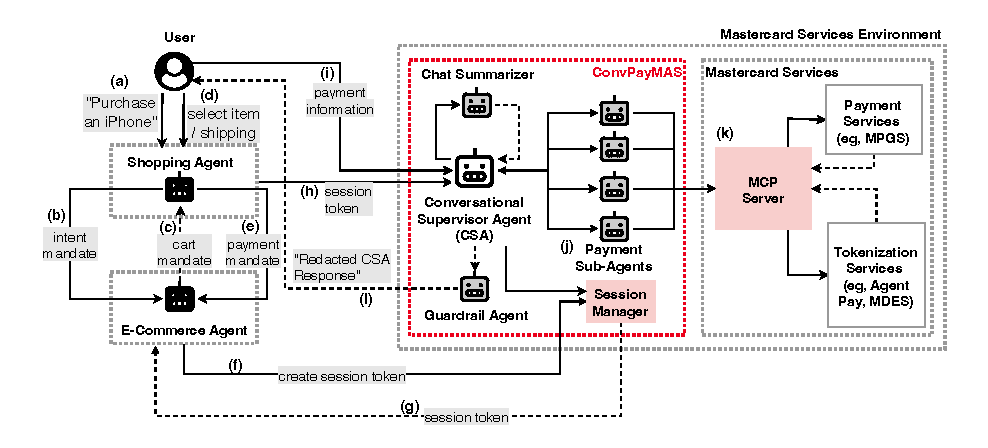
\includegraphics[width=.75\linewidth]{figures/SystemArchitecture3.pdf}
    \caption{Overview of the agentic payment ecosystem with ConvPayMAS.}
    \label{fig:architecture}
\end{figure*}

To address these challenges, we propose the \textbf{\emph{LLM-Based Conversational Payment Multi-Agent System} (ConvPayMAS)}, which abstracts payment-rail complexity within a specialized multi-agent architecture. In this demonstration\footnote{Demo video URL: \url{https://vimeo.com/1152577656}}, we show how ConvPayMAS interoperates with other agents in an agentic payment environment to enable practical conversational commerce. Our key contributions are firstly, a \textbf{single entry point for payment.} ConvPayMAS exposes a \emph{Conversational Supervisor Agent} (CSA) as a unified interface via standardized protocols, enabling external agents to access Mastercard payment functions without integrating multiple APIs. Next, we \textbf{isolate PCI's scope}, where sensitive payment handling occurs within ConvPayMAS, allowing external agents to delegate payment to the CSA without touching sensitive cardholder data. Lastly, we create an \textbf{end-to-end conversational flow}, as ConvPayMAS keeps the payment journey within the conversational loop, reducing chat-to-checkout context switching from product discovery through payment confirmation.

\section{Methodology and System Design}

This section describes the agentic payment architecture (Fig.~\ref{fig:architecture}) and the design of ConvPayMAS. The system comprises three top-level agents that communicate via standardized protocols: \textbf{(1) ConvPayMAS}, a secure server-side agent providing a conversational interface for payment processing; \textbf{(2) Shopper Agent}, a user-side assistant that interprets intent and navigates marketplaces; and \textbf{(3) E-commerce Agent}, a merchant-side agent that handles catalog queries, cart operations, and payment initiation via ConvPayMAS.

\subsection{ConvPayMAS Design}
\label{methodoloty_convpaymas_design}

ConvPayMAS adopts a hierarchical modular architecture for deterministic payment execution, orchestrated with LangGraph~\cite{langchain2024langgraph}.
\textbf{Conversational Supervisor Agent (CSA).}
The CSA is the sole entry point for external agents. It parses natural-language requests and delegates execution to internal sub-agents.

\textbf{Payment Sub-Agents.}
ConvPayMAS employs five specialized sub-agents (Fig.~\ref{fig:architecture}f) using \textbf{role-based protocols}~\cite{hong2024metagpt, tran2025mascollab, guo2024mascollab}:
\textbf{List Card} retrieves masked PANs from the wallet;
\textbf{Create Card} accepts encrypted card data (AES-256-CBC) and initiates OTP;
\textbf{Validate Card} verifies OTP to activate cards;
\textbf{Charge Card} executes transactions;
\textbf{Recommender} suggests optimal cards for the transaction.
A \textbf{Chat Summarizer} compresses conversation history within bounded context windows.
While the current implementation focuses on card payment, ConvPayMAS is designed to be extensible to additional payment rails (e.g., bank-account transfers or stablecoin-based payment) by swapping or adding function-specific sub-agents and MCP tools behind the same conversational interface.

\textbf{MCP Server Tools.}
ConvPayMAS exposes MCP~\cite{anthropic2024mcp} tools for card registration, session management, and payment operations, enabling secure tokenization, real-time authorization, and wallet management through Mastercard's payment infrastructure.

\subsection{Security and Protocol Design}

\textbf{Agent-to-Agent Protocol -}
We use Google’s Agent2Agent (A2A) protocol~\cite{google2025a2a} for trusted and secure inter-agent communication. Messages are protected with AES-256-CBC using session keys, and sessions are managed with JWT (HS256). \textbf{Three-Mandate Verification -} We implement Google’s Agent Payment Protocol (AP2)~\cite{google2025ap2} using three mandates: an \textit{Intent Mandate} capturing purchase intent; a merchant-signed \textit{Cart Mandate}; and a \textit{Payment Mandate} binding user authorization to the cart via a hash chain for verifiable dispute resolution. \textbf{Card Data Security -} Card data (PAN, CVV, expiry) is encrypted client-side with AES-256-CBC. The MCP server issues per-session keys. PANs are validated with a Luhn check and expiry dates are verified before wallet storage. A Guardrail Agent redacts PCI/PII from conversation logs before any external transmission.


\subsection{Payment Flow and Live Demonstration}
The demonstration presents the below transaction flow live, with scenarios for mandate verification, card security, and multi-agent coordination. The transaction journey proceeds through four phases:


\textbf{Phase 1 -- Intent \& Discovery.}
The user expresses intent to the Shopper Agent (e.g., ``Purchase an iPhone'') (Fig.~\ref{fig:architecture}a). The Shopper Agent creates an \textit{IntentMandate} and sends it to the E-commerce Agent via A2A streaming (Fig.~\ref{fig:architecture}b). The merchant searches inventory and returns a signed \textit{CartMandate} (Fig.~\ref{fig:architecture}c) with items, prices, and shipping options—digitally signed with HMAC-SHA256. If there are price modifications, a new \textit{CartMandate} must be signed.

\textbf{Phase 2 - Selection \& Payment Mandate:} The user selects an item and shipping method (Fig.~\ref{fig:architecture}d). The Shopper Agent creates a \textit{PaymentMandate} containing a JWT that references the Cart Mandate's authorization and the hashed payment contents.

\textbf{Phase 3 - Session Creation:} The E-commerce Agent receives the \textit{PaymentMandate} (Fig.~\ref{fig:architecture}e) via A2A and validates all three mandates' cryptographic integrity—verifying JWT signatures, expiry times, audience claims, and hash chain. Upon validation, it creates a transaction session (Fig.~\ref{fig:architecture}f), returning a session token (Fig.~\ref{fig:architecture}g).

\textbf{Phase 4 - Payment Execution:} The user is handed off to ConvPayMAS with the session token (Fig.~\ref{fig:architecture}h, i). The CSA routes requests to appropriate sub-agents (Fig.~\ref{fig:architecture}j)—\textit{List Card, Create Card, Validate Card, Charge Card}—which invoke MCP server tools for payment processing (Fig.~\ref{fig:architecture}k). Upon completion, the CSA returns confirmation via natural language (Fig.~\ref{fig:architecture}l).


%%%%%%%%%%%%%%%%%%%%%%%%%%%%%%%%%%%%%%%%%%%%%%%%%%%%%%%%%%%%%%%%%%%%%%%%
%%% PAGE 3: REFERENCES
%%%%%%%%%%%%%%%%%%%%%%%%%%%%%%%%%%%%%%%%%%%%%%%%%%%%%%%%%%%%%%%%%%%%%%%%

\clearpage
\section{Acknowledgments}
This work was supported by Mastercard Foundry R\&D. The authors thank Anamika Thokal and Varuna Ektare from the Mastercard Foundry Pune R\&D team for their assistance with the demonstration video and program management, respectively.
This work was also supported by the EngD Program at Singapore Management University.
\bibliographystyle{ACM-Reference-Format}
\bibliography{references}

\iffalse
%%%%%%%%%%%%%%%%%%%%%%%%%%%%%%%%%%%%%%%%%%%%%%%%%%%%%%%%%%%%%%%%%%%%%%%%
%%% PAGE 4: DEMONSTRATION REQUIREMENTS
%%%%%%%%%%%%%%%%%%%%%%%%%%%%%%%%%%%%%%%%%%%%%%%%%%%%%%%%%%%%%%%%%%%%%%%%
\clearpage
\section*{Demonstration Requirements}

This section specifies the technical and logistical requirements for the demonstration setup at the AAMAS 2026 conference.

\subsection*{Space Requirements}
\begin{itemize}
    \item Standard demonstration booth space% (approximately 2m $\times$ 2m)
    \item One table for laptop display and demonstration materials
    \item Two chairs for demonstrators
    \item 2 Poster stands for architectural diagram display (A0 size)
\end{itemize}

\subsection*{Equipment (Provided by Demonstrators)}
\begin{itemize}
    \item \textbf{Laptop:} MacBook Pro with Apple Silicon (M-series) with 64GB+ RAM for running the multi-agent system locally
    \item \textbf{External Monitor:} 24" or bigger display for audience visibility during live demonstrations
    \item \textbf{Backup Device:} Secondary laptop with pre-recorded demonstration video in case of technical issues
\end{itemize}

\subsection*{Equipment (Required from Venue)}
\begin{itemize}
    \item \textbf{Power:} Two standard power outlets (Type G for Cyprus, or universal adapters will be provided)
    \item \textbf{Internet:} Stable WiFi connection with minimum 10 Mbps bandwidth for LLM API calls (OpenAI GPT-4o, Anthropic Claude)
    \item \textbf{Poster Stand:} Two standard poster stands for A0 portrait poster
\end{itemize}

\subsection*{Software Stack}
The demonstration runs four microservices locally:
\begin{itemize}
    \item \textbf{ConvPayMAS MCP Server} (Port 8080): FastMCP-based payment tools server with SQLite persistence for cards, sessions, and mandates
    \item \textbf{ConvPayMAS A2A Agent} (Port 8003): LangGraph-orchestrated payment agent with Supervisor, List Card, Create Card, Validate Card, Charge Card, and Recommender sub-agents
    \item \textbf{E-commerce Agent} (Port 8090): Merchant catalog and cart management with Catalog Agent and mandate signing
    \item \textbf{Shopper Agent} (Port 8002): User-facing shopping assistant with Discovery, Address, and main Shopper sub-agents
\end{itemize}

All services use Python 3.13 with LangGraph for orchestration and the A2A SDK for inter-agent communication. The system requires API keys for OpenAI (GPT-4o models), with optional Anthropic and Google API keys for model diversity demonstrations.

\subsection*{Demonstration Scenarios}
We demonstrate the following interactive scenarios to validate the framework:
\begin{enumerate}
    \item \textbf{End-to-End Shopping Flow:} User initiates a budget-constrained query (``Buy MacBook under \$2,000'') $\rightarrow$ Shopper Agent creates \textit{IntentMandate} $\rightarrow$ E-commerce Agent returns signed \textit{CartMandate} with SKU options $\rightarrow$ User selects item and shipping preference $\rightarrow$ \textit{PaymentMandate} created via chain-of-hashes $\rightarrow$ Secure handover to ConvPayMAS for new card entry and OTP verification $\rightarrow$ Transaction finalized with order confirmation.
    
    \item \textbf{Mandate Verification:} Live demonstration of the AP2 three-mandate cryptographic chain, featuring JWT signing with HMAC-SHA256, audience verification, and real-time validation of the hash chain integrity.
    
    \item \textbf{Card Security:} Demonstration of AES-256-CBC encrypted card transmission, Luhn algorithm validation, and the OTP verification flow required to transition the card state from \texttt{PENDING} to \texttt{ACTIVE}.
    
    \item \textbf{Multi-Agent Coordination:} Visualization of A2A protocol messages (Agent Cards, streaming requests, \textit{TaskStatusUpdateEvent}) and LangGraph state transitions occurring during a live transaction.
    
\end{enumerate}

\subsection*{Contingency Plans}
\begin{itemize}
    \item Pre-recorded video demonstration (10 minutes) available offline covering all four scenarios
    \item Local LLM fallback using Ollama with Llama models if API connectivity issues occur
    \item Static architectural walkthrough using poster if live system is unavailable
\end{itemize}

\subsection*{Accessibility}
\begin{itemize}
    \item Demonstration screen will be positioned at standing height for visibility
    \item Large font terminal output for command-line demonstrations
    \item Printed handouts with QR codes linking to project repository and documentation
\end{itemize}
\fi

%%%%%%%%%%%%%%%%%%%%%%%%%%%%%%%%%%%%%%%%%%%%%%%%%%%%%%%%%%%%%%%%%%%%%%%%
\label{TotPages}

\end{document}


